
\section{Implementering}
\label{sec:implementering}

\subsection{Kretskort}

For å kunne gjøre systemet å kompakt som mulig bestemte vi oss for å benytte et kretskort for å sende signalene fra mikrokontrolleren til OLED-skjermen. Kretskortet gjør designet kompakt for brukeren, samtidig at komponentene vil sitte bedre og dermed bli bedre rustet for bevegelser. 

En viktig del av systemet er kommunikasjon mellom enheten og serveren. Dette foregår over WiFi, ettersom det gir en stabil tilkobling og det blir da mulig med flere enheter koblet til samme server. For å benytte WiFi, brukes en mikrokontroller av type ESP32, med innebygd WiFi-modul. 

\begin{figure}[H]
    \centering
    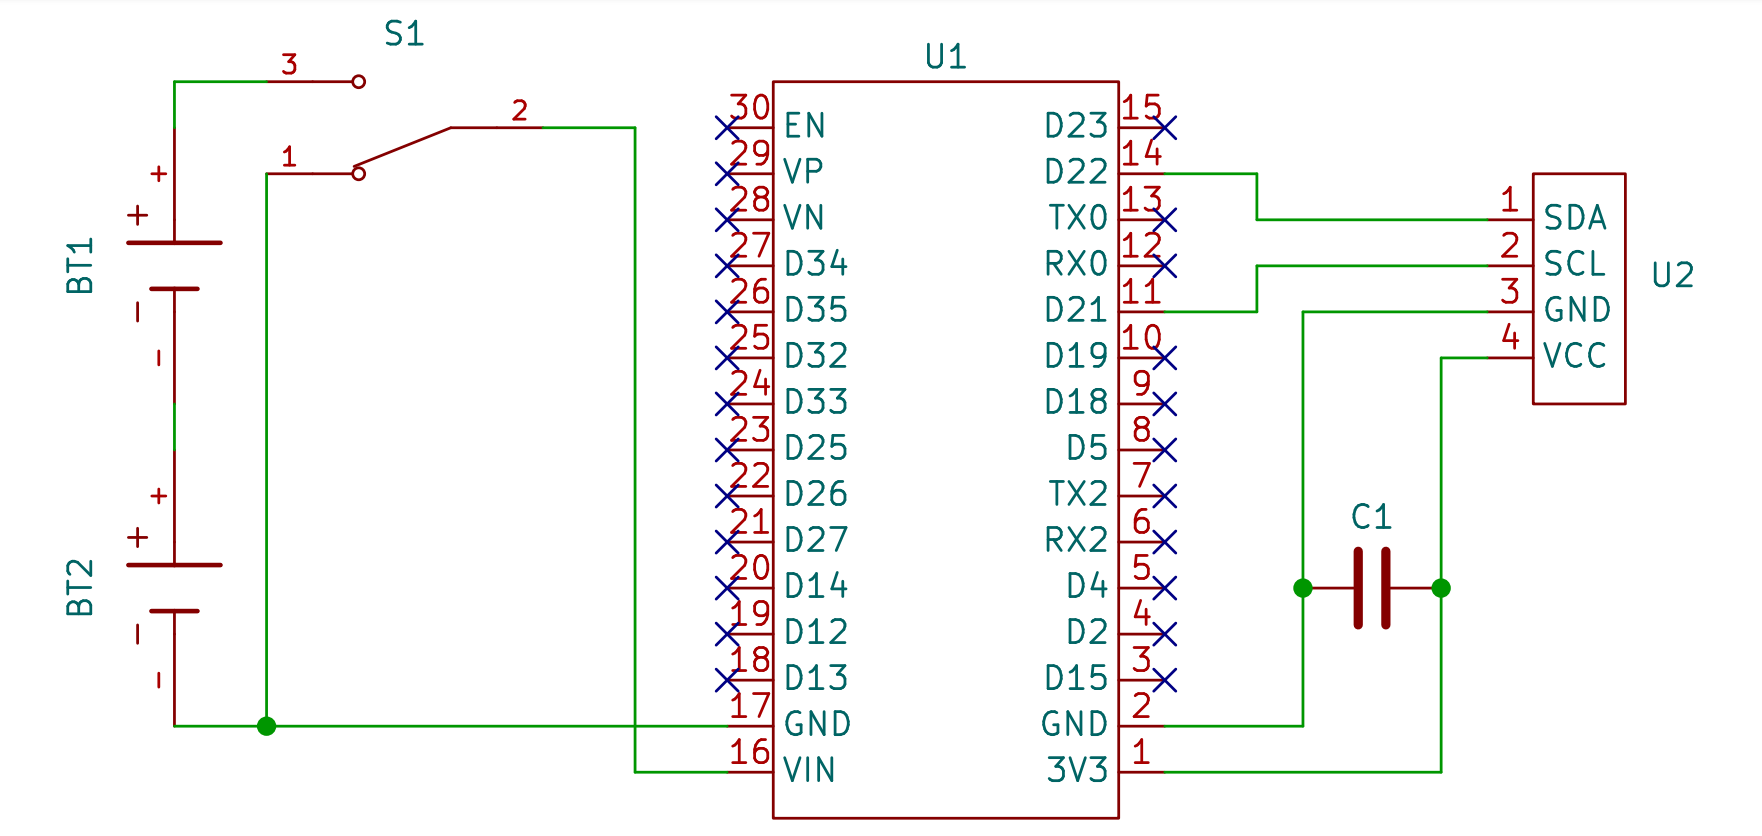
\includegraphics[width=0.8\textwidth]{rapport/Images/implementering/Kretskort tegning.png}
    \caption{Kretstegning}
    \label{fig:kretskort-kretstegning}
\end{figure}

Som vist i figur \ref{fig:kretskort-kretstegning}, består kretsen av to batterier, som er koblet til en bryter, S1. Bryteren gir strøm til U1, som er mikrokontrolleren, som gir brukeren mulighet til å skru av og på systemet. Ut fra U1 går det 4 ledninger, to for strøm og to for data. Disse går til U2, som er skjermen. Kondensatoren C1 er koblet mellom jord og 3V3 for å beskytte mikrokontrolleren ved uventede spenningsfall fra batteriet eller ved raske endringer gitt av bryteren.

Årsaken til at vi har brukt to batterier er at ettersom vi ønsker et kompakt system, for å bedre brukeropplevelsen, har vi valgt CR2032 batterier. Disse har en spenning på 3V, noe som blir for lite for å kunne drive systemet. Ved å parallellkoble to slike batterier, vil vi ha 6V, som er nok til å drive mikrokontrolleren og OLED-skjermen. 

Ved design av en kompakt PCB, hvor alle komponentene er inkludert, vil den se noe ut som vist i figur \ref{fig:kretskort forside uten komponenter} og \ref{fig:kretskort bakside uten komponenter}. \\
\begin{minipage}{\linewidth}
    \centering
    \begin{minipage}{0.45\linewidth}
      \begin{figure}[H]
          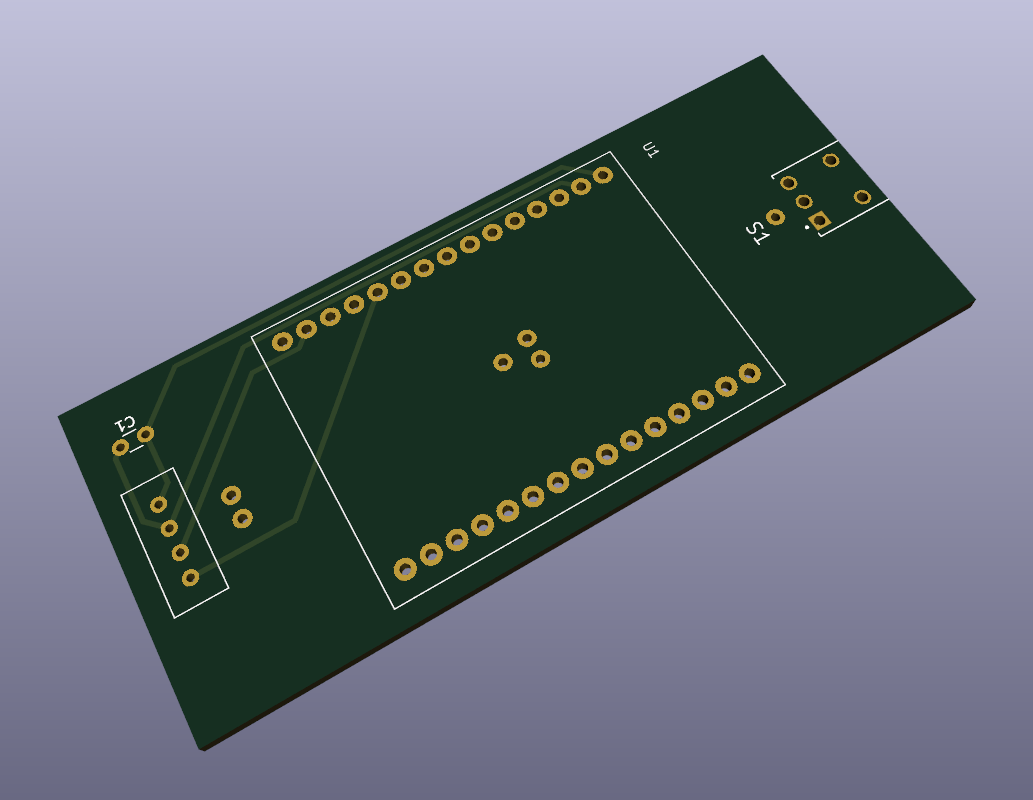
\includegraphics[width=\linewidth]{rapport/Images/implementering/PCB front.png}
          \caption{Kretskort forside}
          \label{fig:kretskort forside uten komponenter}
      \end{figure}
    \end{minipage}
    \hspace{0.05\linewidth}
    \begin{minipage}{0.45\linewidth}
      \begin{figure}[H]
          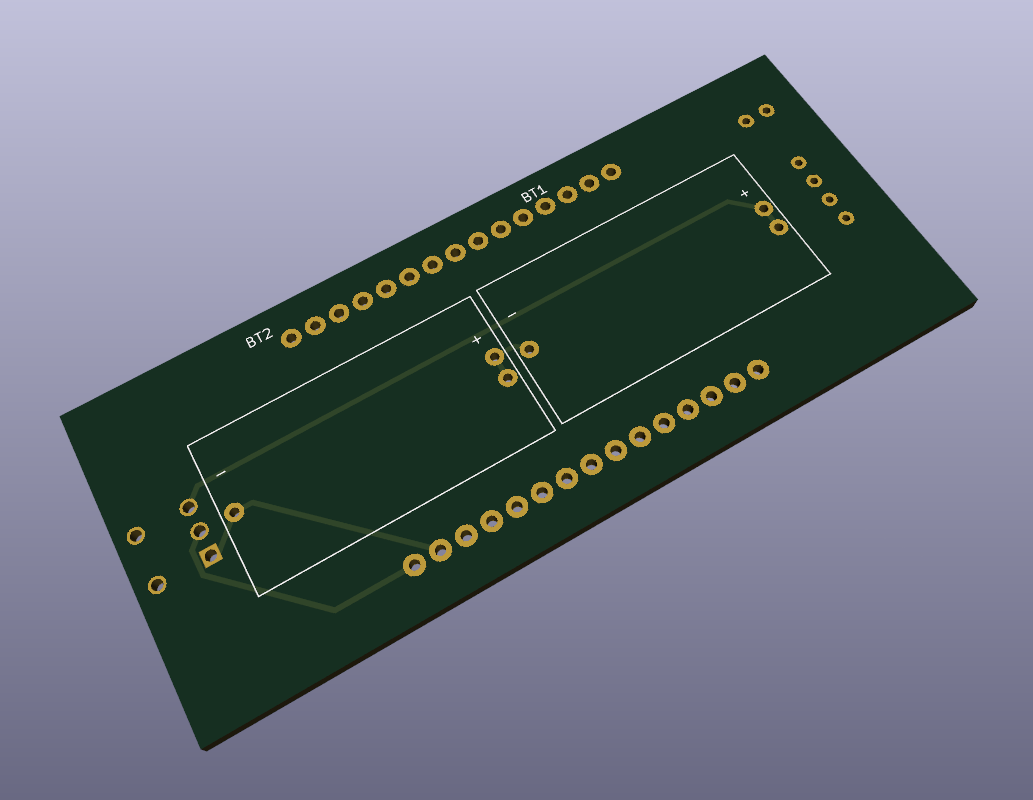
\includegraphics[width=\linewidth]{rapport/Images/implementering/PCB back.png}
          \caption{Kretskort bakside}
          \label{fig:kretskort bakside uten komponenter}
      \end{figure}
    \end{minipage}
  \end{minipage}

Ved 3D modellering, kan man få et inntrykk av hvordan kretskortet vil se ut til slutt. Dette er vist under i figur \ref{fig:kretskort forside med komponenter} og \ref{fig:kretskort bakside med komponenter}. \\ 
\begin{minipage}{\linewidth}
    \centering
    \begin{minipage}{0.45\linewidth}
      \begin{figure}[H]
          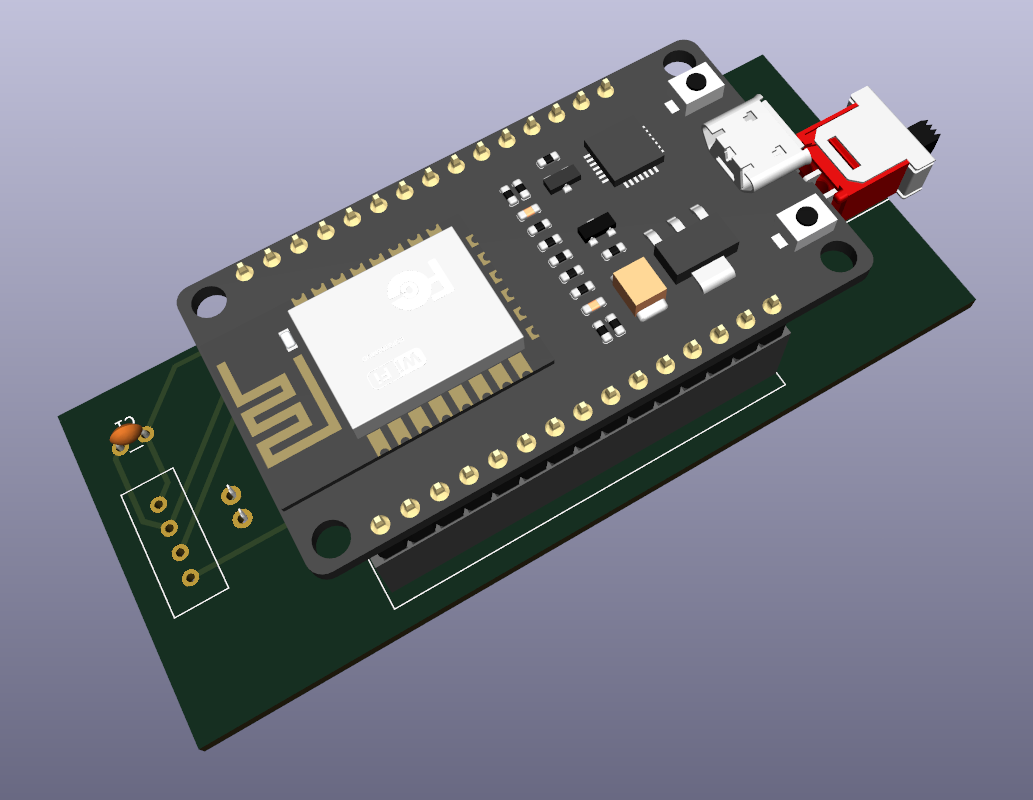
\includegraphics[width=\linewidth]{rapport/Images/implementering/PCB 3D front.png}
          \caption{3D modellert kretskort forside}
          \label{fig:kretskort forside med komponenter}
      \end{figure}
    \end{minipage}
    \hspace{0.05\linewidth}
    \begin{minipage}{0.45\linewidth}
      \begin{figure}[H]
          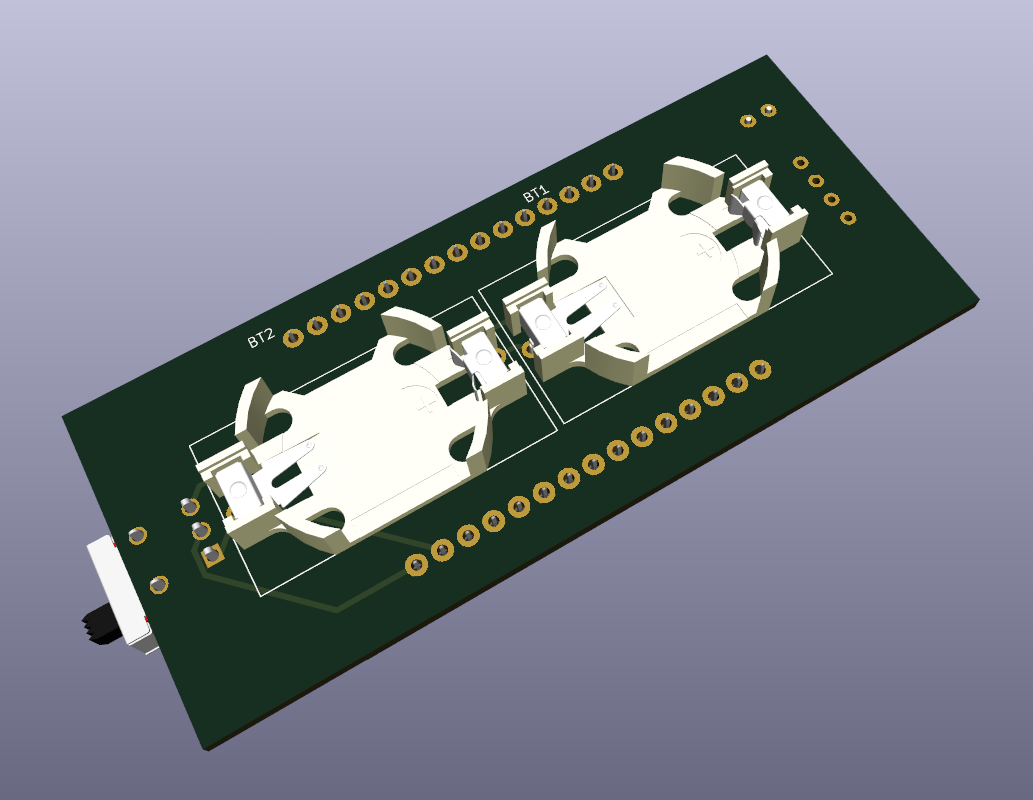
\includegraphics[width=\linewidth]{rapport/Images/implementering/PCB 3D back.png}
          \caption{3D modellert kretskort bakside}
          \label{fig:kretskort bakside med komponenter}
      \end{figure}
    \end{minipage}
  \end{minipage}

